\subsection{Rulebase File}
\label{sec:rbfile}

Des Weiteren kann es sein, dass Sie für eine Domain (hier unser Zustandsautomat) mehrere Regelbasen zur Verfügung stellen möchten.
Das ist z.B. dann der Fall, wenn man sich die Editierregeln mittels Generator hat generieren lassen und einige jetzt noch manuell nachgebessert oder ergänzt werden müssen.
Um eine neue Regelbasis zu erstellen, gehen Sie wieder auf \texttt{File} $\triangleright$ \texttt{New} $\triangleright$ \texttt{Other...} und wählen Sie  \texttt{SiLift} $\triangleright$ \texttt{Rulebase File}

\begin{figure}[H]
\centering
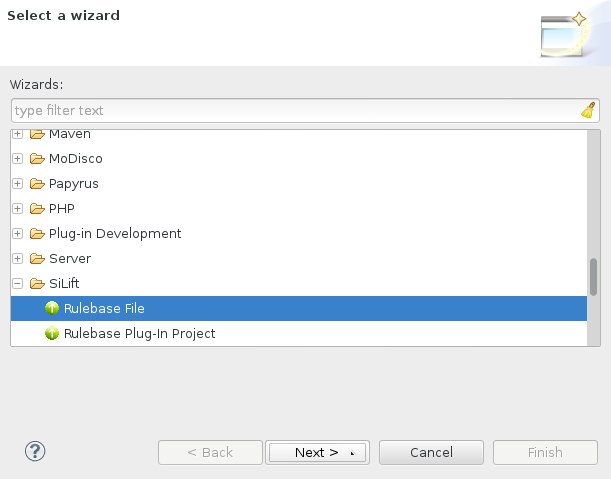
\includegraphics[width=0.6\textwidth]{recognitionrules/graphics/silift-wizard_rulebase_file_page01.png}
\caption{Erstellen einer neuen Regelbasis}
\label{silift-wizard_rulebase_file_page01}
\end{figure}

Im nächsten Schritt wählen Sie das Verzeichnis \texttt{rulebase} des bestehenden Projekts für die Erkennungsregeln und geben der Regelbasis einen Namen (vgl. Abb. \ref{silift-wizard_rulebase_file_page02}).

\begin{figure}[H]
\centering
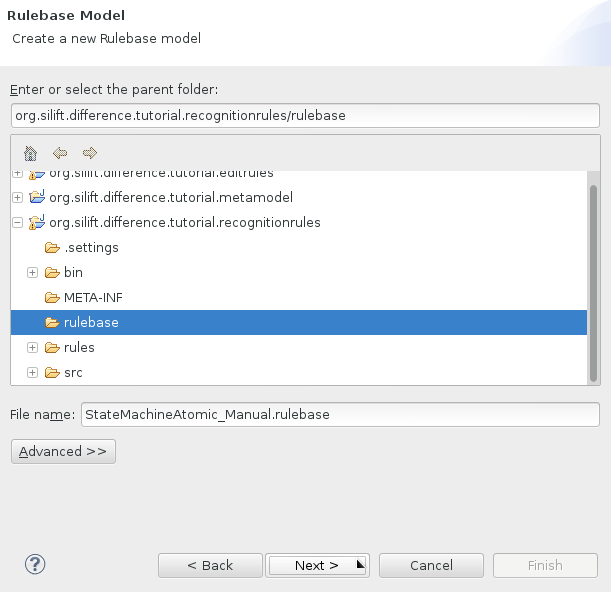
\includegraphics[width=0.6\textwidth]{recognitionrules/graphics/silift-wizard_rulebase_file_page02.png}
\caption{Erstellen einer neuen Regelbasis}
\label{silift-wizard_rulebase_file_page02}
\end{figure}

Jetzt wählen Sie wie bereits zuvor die gewünschten Editierregeln aus und klicken auf \texttt{Finish} (vgl. Abb. \ref{silift-wizard_rulebase_file_page03}).

\begin{figure}[H]
\centering
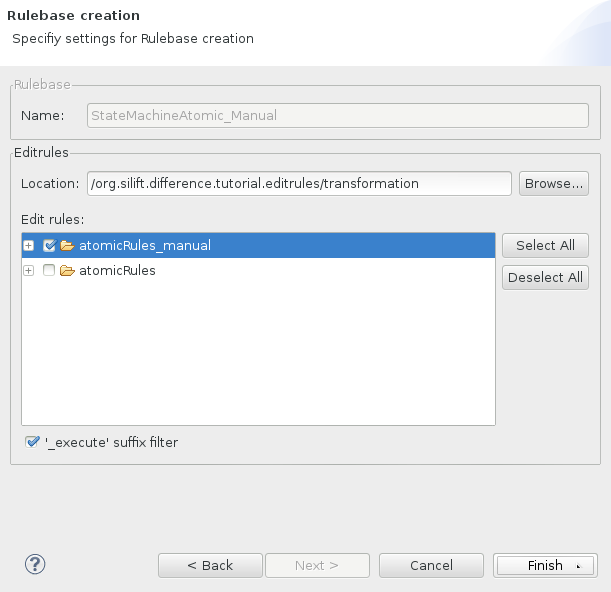
\includegraphics[width=0.6\textwidth]{recognitionrules/graphics/silift-wizard_rulebase_file_page03.png}
\caption{Erstellen einer neuen Regelbasis}
\label{silift-wizard_rulebase_file_page03}
\end{figure}

Damit haben Sie Ihrem Projekt eine neue Regelbasis hinzugefügt (vgl. Abb. \ref{silift-rulebase_package_explorer}).
Als nächstes muss sich diese Regelbasis noch als Erweiterung (engl. \textit{Extension}) bei dem Plugin registrieren.


\begin{figure}[H]
\centering
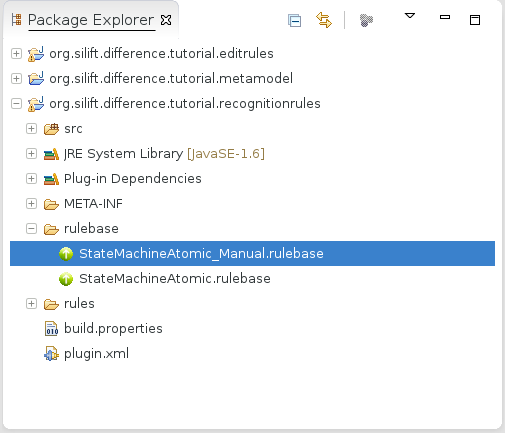
\includegraphics[width=0.3\textwidth]{recognitionrules/graphics/silift-rulebase_package_explorer.png}
\caption{Package Explorer: Regelbasen}
\label{silift-rulebase_package_explorer}
\end{figure}

Öffnen Sie das Verzeichnis \texttt{src} über den \textit{Package Explorer}, kopieren Sie die bereits existierende Klasse und nennen diese entsprechend um (vgl. Abb. \ref{silift-rulebase_class}).
Danach öffnen Sie die Klasse und passen den Wert der Variablen \texttt{RULE\_BASE\_NAME} entsprechend an. 

\begin{figure}[H]
\centering
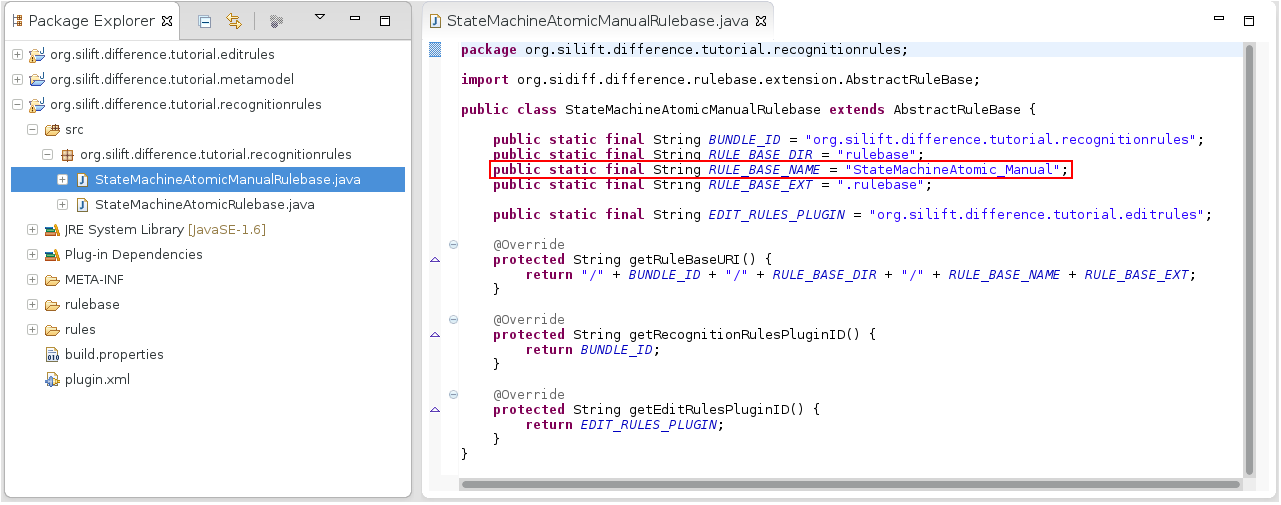
\includegraphics[width=0.8\textwidth]{recognitionrules/graphics/silift-rulebase_class.png}
\caption{Klasse: StateMachine\_AtomicManualRulebase}
\label{silift-rulebase_class}
\end{figure}

Öffnen Sie die \texttt{MANIFEST.MF} und wählen Sie den Reiter \texttt{Extensions} aus. 
Klicken Sie auf \texttt{Add...} und selektieren Sie den \textit{Extension Point} \texttt{org"".""sidiff"".""difference"".""rulebase"".""rulebase""\_extension}. Klicken Sie auf \texttt{Finish} (vgl. Abschnitt \ref{sec:own_matching_engine}).\\
Wechseln Sie danach in den Reiter \texttt{plugin.xml} und fügen Sie dem eben erstellen Extension Point die entsprechende URI der Erweiterung bei (vgl. Abb. \ref{silift-plugin_rulebase_manifest_plugin}).

\begin{figure}[H]
\centering
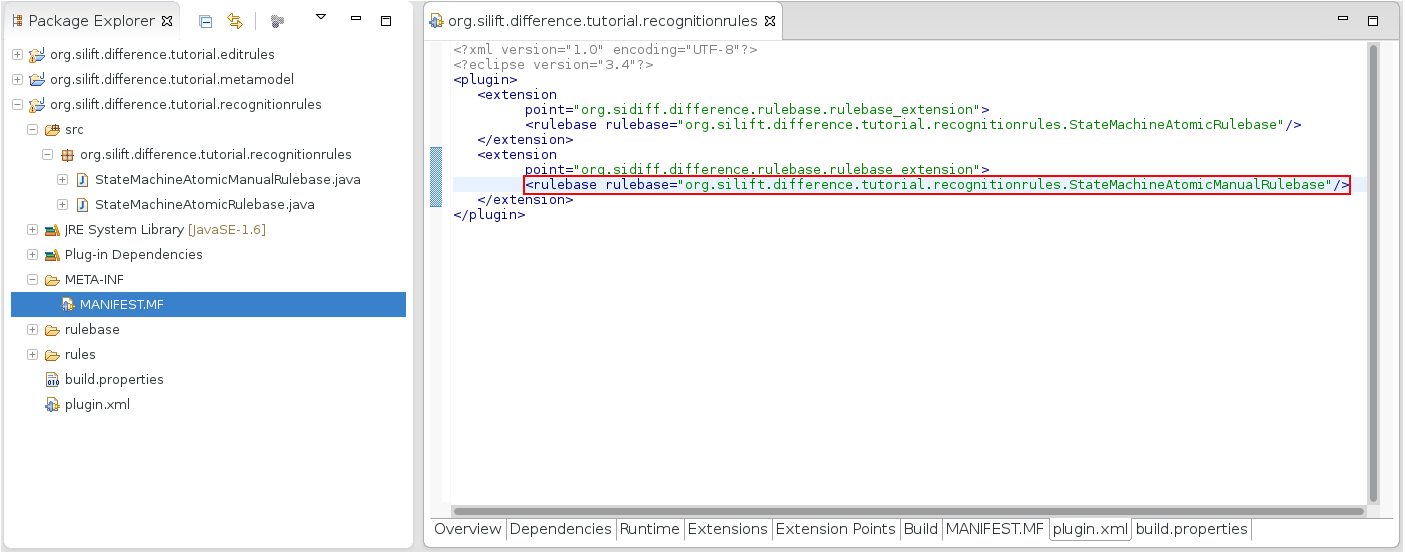
\includegraphics[width=0.8\textwidth]{recognitionrules/graphics/silift-plugin_rulebase_manifest_plugin.png}
\caption{Manifest.MF: \texttt{plugin.xml}}
\label{silift-plugin_rulebase_manifest_plugin}
\end{figure}

